\section{The Beale Function}
\label{sec:beale_function}

  Introduced by Beale in 1958\footnote{
    Beale, E. M. (1958). \enquote{On an Iterative Method for Finding a Local 
    Minimum of a Function of More than One Variable}. 
  }, the Beale function is a multimodal function with sharp peaks at the corners
  of the domain.

  \begin{definition}[Beale function]
    \label{def:beale_function}
    The \emph{Beale function}, denoted as \(f: \mathbb{R}^2 \rightarrow 
    \mathbb{R}\), is defined by the following equation:

    \begin{equation}
    \label{eq:beale_function}
      f(x,\,y) = (1.5 - x + xy)^2 + (2.25 - x + xy^2)^2 + (2.625 - x + xy^3)^2
    \end{equation}

    Where \(x \in [-4.5,\,4.5]\) and \(y \in [-4.5,\,4.5]\).
  \end{definition}

  The Beale function's global minima is located at \(f(3,\,0.5) = 0\).
  A contour plot and a surface plot of the Beale function are shown in
  \vref{fig:beale_function}.

  % \begin{figure}[ht!]
  %   \centering
  %   \begin{subfigure}[b]{0.4\textwidth}
  %     \centering
  %     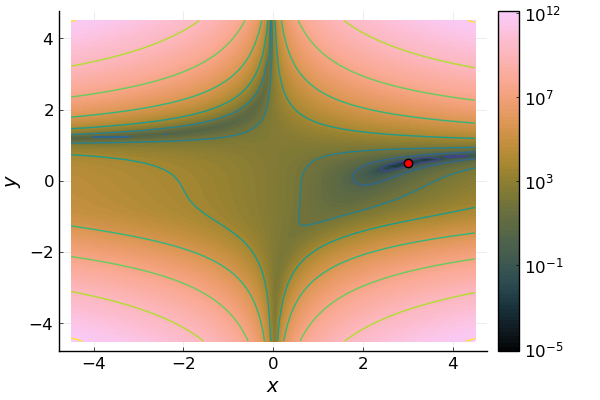
\includegraphics[width=\textwidth]{img/test_functions/beale_contour.png}
  %   \end{subfigure}
  %   \begin{subfigure}[b]{0.4\textwidth}
  %     \centering
  %     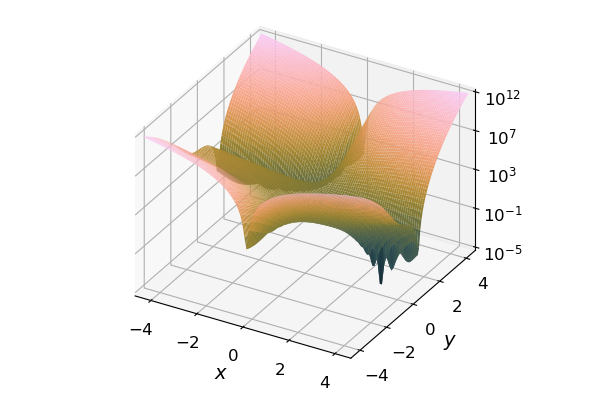
\includegraphics[width=\textwidth]{img/test_functions/beale_surface.png}
  %   \end{subfigure}
  %   \caption{Beale Function}
  %   \label{fig:beale_function}
  % \end{figure}